% !TEX TS-program = pdflatex
% !TEX encoding = UTF-8 Unicode

% This is a simple template for a LaTeX document using the "article" class.
% See "book", "report", "letter" for other types of document.

\documentclass[11pt]{article} % use larger type; default would be 10pt

\usepackage[utf8]{inputenc} % set input encoding (not needed with XeLaTeX)

%%% Examples of Article customizations
% These packages are optional, depending whether you want the features they provide.
% See the LaTeX Companion or other references for full information.

%%% PAGE DIMENSIONS
\usepackage{geometry} % to change the page dimensions
\geometry{a4paper} % or letterpaper (US) or a5paper or....
% \geometry{margin=2in} % for example, change the margins to 2 inches all round
% \geometry{landscape} % set up the page for landscape
%   read geometry.pdf for detailed page layout information

\usepackage{graphicx} % support the \includegraphics command and options

% \usepackage[parfill]{parskip} % Activate to begin paragraphs with an empty line rather than an indent

%%% PACKAGES
\usepackage{booktabs} % for much better looking tables
\usepackage{array} % for better arrays (eg matrices) in maths
\usepackage{paralist} % very flexible & customisable lists (eg. enumerate/itemize, etc.)
\usepackage{verbatim} % adds environment for commenting out blocks of text & for better verbatim
\usepackage{subfig} % make it possible to include more than one captioned figure/table in a single float
\usepackage{multicol,caption}
\usepackage{wrapfig}
% These packages are all incorporated in the memoir class to one degree or another...

%%% HEADERS & FOOTERS
\usepackage{fancyhdr} % This should be set AFTER setting up the page geometry
\pagestyle{fancy} % options: empty , plain , fancy
\renewcommand{\headrulewidth}{0pt} % customise the layout...
\lhead{}\chead{}\rhead{}
\lfoot{}\cfoot{\thepage}\rfoot{}

%%% SECTION TITLE APPEARANCE
\usepackage{sectsty}
\allsectionsfont{\sffamily\mdseries\upshape} % (See the fntguide.pdf for font help)
% (This matches ConTeXt defaults)

%%% ToC (table of contents) APPEARANCE
\usepackage[nottoc,notlof,notlot]{tocbibind} % Put the bibliography in the ToC
\usepackage[titles,subfigure]{tocloft} % Alter the style of the Table of Contents
\renewcommand{\cftsecfont}{\rmfamily\mdseries\upshape}
\renewcommand{\cftsecpagefont}{\rmfamily\mdseries\upshape} % No bold!
\newcommand{\squeezeup}{\vspace{-25pt}}
\newenvironment{Figure}{\par\medskip\noindent\minipage{\linewidth}}{\endminipage\par\medskip}
\newenvironment{Table}{\par\smallskip\noindent\minipage{\linewidth}}{\endminipage\par\smallskip}
%%% END Article customizations

%%% The "real" document content comes below...

\title{Homework 1 : Supervised Deep Learning}
\author{João Ramos da Silva Tabuaço Freitas \\ Università Degli Studi di Padova \\ Student ID: 2009440}
\date{18 July 2022} % Activate to display a given date or no date (if empty),
         % otherwise the current date is printed 

\begin{document}
\maketitle
\begin{multicols}{2}
[
\section*{\centering Introduction}
Supervised learning comprises the simplest applications of neural network models with the purpose of classifying data constructed by numerous features. The nature of the task at hand depends on the type of labels associated with the data. Labels forming a continuous set pertain to \textbf{regression} tasks, while data with associated labels forming discrete sets make up \textbf{classification} tasks. In this report, these two tasks are performed by implementing neural network models with the PyTorch framework. A fully connected network is employed for the regression task, while a convolutional one is used to perform the classification. While both tasks are qualified as supervised learning, they differ enough that it is worth addressing them separately. Thus, this report addresses the two tasks separately.
]
\section{Regression}
The goal of the regression task is to learn a single-variable objective function. The model performance is quantified by the mean squared error (MSE) between the model output $\hat{y}$ and the data's respective label $y$. The goal is to find the set of parameters $\{\hat{w}\}$ that minimize the MSE:\\
\begin{equation}
\{\hat{w}\}= \arg\min_{w} \sum_{i = 1}^{n}\left(\hat{y}_i - y_i\right)^{2}
\end{equation}

\noindent MSE is advantageous in comparison to the mean absolute error because it penalizes points that are more correctly classified in a lighter manner, while placing a stronger emphasis on improving the model such that data that lead to a larger loss are prioritized. Traditionally, MSE minimization is implemented with the method of least squares. However, it requires making an assumption about the number of parameters (i.e. choosing an adequate curve to attempt fitting). The advantage of using a deep learning model lies in the large number of degrees of freedom which can, in turn, mimic the behavior of the objective function faithfully with several different configurations of its parameters. Because of that, it is possible that different models yield similarly acceptable results, thus increasing the likelihood of finding an adequate representation of the objective function. While the computational cost of training deep-learning models can quickly increase due to the tensorial nature of the parameters, it is offset by the computational prowess of graphical processing units (GPUs), which are thoroughly used in this exploration.
\subsection{Methods}

A fully-connected neural network is implemented to learn the functional behavior of some unknown finite polynomial. Its architecture consists of three hidden layers. The number of neurons in each layer is tuned through a Bayesian-like parameter search, implemented using the Optuna framework.\\

\noindent The data used in the regression task are divided in a training and a test dataset. Uniform noise is added to the training labels, and significant intervals of the data space are removed. These transformations help combat overfitting. The test data is left unaltered. Because the model is relatively simple, both the training and test sets are composed of $100$ samples.
\begin{Figure}
	\centering
	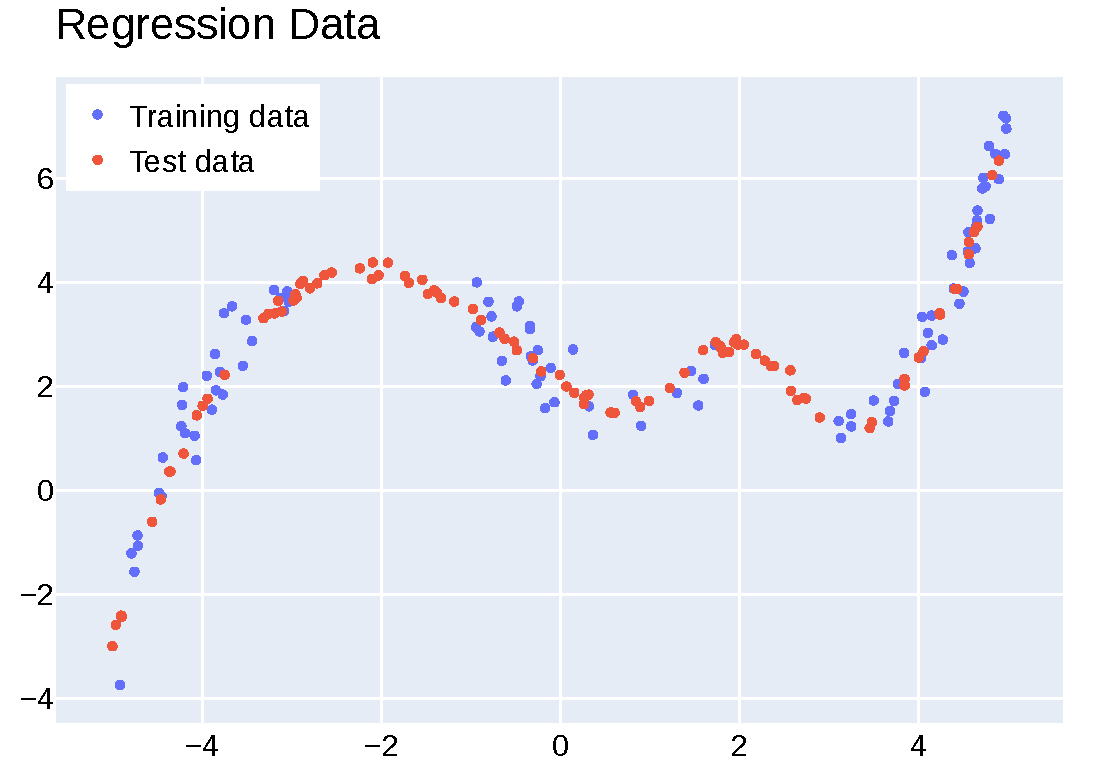
\includegraphics[width=\linewidth]{res/fig0.pdf}
\end{Figure}

\noindent The gaps in the training data will likely be the main drivers of the model's validation loss. Because of that, a combination of regularization techniques will be implemented.\\

\noindent The adequate model architecture was determined by a preliminary random search. This involved randomly sampling 50 architectures. The structure was kept constant: three hidden layers, each with associated neuron drop-out. Each model was preliminarily trained over 200 epochs. The number of neurons in each hidden layer, along with the activation function, optimizer type and respective learning rate were all randomly sampled according to Optuna's TPESampler. This sampler starts out with uniform sampling of hyperparameters, becoming increasingly sensitive to the prior models tested as the grid-search progresses. This strategy offers an adequate compromise between the computationally exhaustive classic grid-search and a completely random search. Naturally, this faces an issue that is quite similar to vanishing gradients: the sampler might keep generating similar architectures that yield loss close to a local minimum, while missing other configurations that could, in theory, perform better. Unfortunately, the nature of the TPESampler means this issue is inevitable. The best preliminary architecture had the following parameters:\\

\begin{Table}
\centering
\begin{tabular}{c|c}
$N_1$ \quad & \quad 127\\
$N_2$ \quad & \quad 168\\
$N_3$ \quad & \quad 80\\
Activation \quad & \quad ReLU\\
Dropout \quad & \quad 0.019\\
Optimizer \quad & \quad Adam\\
\end{tabular}
\end{Table}

\noindent A new model with these parameters is then initialized with the Glorot scheme.
\subsection{Results}
Upon finding a set of best parameters, the model was reinstantiated with those, and trained using K-fold cross-validation, with 5 folds of the training data. Each training was performed over 400 epochs. 

\begin{Figure}
	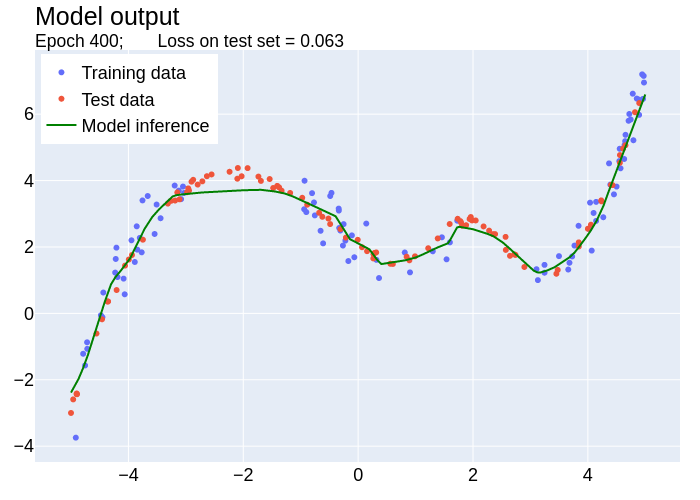
\includegraphics[width=\linewidth]{res/newplot.png}
\end{Figure}
%%%%%%%%%%%%%HERE

\section{Classification}
The classification task aims to train a model to categorically classify input data. Its most common form consists in classifying a set of images. The raw data consists of pixel values in some given shape, grouped in one or multiple channels. These are normally pre-processed, with several possible objectives ranging from data augmentation to promoting model regularization.

\subsection{Methods}
YAYAYA
involves the analysis of the well-known FashionMNIST dataset, a variation from the standard handwritten digit dataset MNIST. The data consist of images of shape $(1 \times 28 \times 28)$ representing different articles of clothing, in black and white. The categorical nature of the data motivates encoding labels in a discrete manner.\\
\subsection{Results}

More text.

\end{multicols}
\end{document}
